%!TEX root = ../Demo.tex
\chapter{测试内容}

本章内容为测试过程中发现的问题,以及如何修复(部分)这些问题。

% \begin{remark}
%     因为$DFA$的最小化建立在状态等价性的基础之上,所以本文并未专门针对等价性进行测试。    
% \end{remark}



%%%%%%%%%%%%%%%%%%%%%%%%%%%%%%%%%%%%%%%%%%%%%%%%%%%%%%%%%%%%%%%%%%%%%%%%%%%%%%%%%%%%%%%%%%%%%%%%%%%%%%%%%%%%%%%%%%%%%%%%%%%%%%%%%%%%%%%%%%%%%%%%%
\section{无限循环}

按 \ref{sec:get_a_dfa} 节那样实例化一个如表 \ref{tab:DFA4} 的 $DFA$ 的对象之后,调用函数 $DFA::min\_Watson()$ 。(表 \ref{tab:DFA4} 对应的状态转移图为图 \ref{fig:DFA4_0},含有陷阱状态 $q_5$ \footnote{进入此状态之后无法通过任何转移离开,如图 \ref{fig:DFA4_0} 中的状态 {$q_5$}。} )

\begin{table}[!htbp]
    \caption{接受{$\mathcal{L}=0^*10^*$}的自动机{\cite{book1}}}
    \label{tab:DFA4}
    \centering
    \small% fontsize
    \setlength{\tabcolsep}{4pt}% column separation
    \renewcommand{\arraystretch}{1.2}%row space 
    %\begin{tabular}{lcrr} 
        \begin{tabular}{l p{3em}<{\centering} p{3em}<{\centering} p{3em}<{\centering}}
        \toprule %\hline 
        \multirow{2}{*}{状态说明} & \multirow{2}{*}{状态} & \multicolumn{2}{c}{输入字符} \\
		\cline{3-4}      &    &$0$ & $1$  \\
        \midrule%\hline
        开始状态(start)  & $q_0$ & $q_1$   & $q_2$   \\
                        & $q_1$ & $q_0$   & $q_3$   \\
        结束状态(accept) & $q_2$ & $q_4$   & $q_5$   \\
        结束状态(accept) & $q_3$ & $q_4$   & $q_5$   \\
        结束状态(accept) & $q_4$ & $q_4$   & $q_5$   \\
        陷阱状态(sink) & $q_5$ & $q_5$   & $q_5$   \\
        \bottomrule%\hline 
    \end{tabular}
\end{table}

% {\bfseries 运行结果:} 函数进入无限循环
\subsection{运行结果}
函数进入无限循环。

% {\bfseries 错误原因:}
\subsection{错误原因} 

单步调试发现进入无限循环的位置为min-bww.cpp(124行),为代码 \ref{lst:minbww} 中的“H.equivalize(p, q);”。
\lstset{style=mystyle}
\begin{lstlisting}[language=C++,label={lst:minbww},caption={min-bww.cpp}]
if (are_eq(p, q, S, H, Z))
{
    // p and q are equivalent.
    H.equivalize(p, q);
}
\end{lstlisting}
单步进入该函数,可以看到代码 \ref{lst:StateEqRel} (StateEqRel.cpp(42行))
\lstset{style=mystyle}
\begin{lstlisting}[language=C++,label={lst:StateEqRel},caption={StateEqRel.cpp}]
for (oldq->iter_start(i); !oldq->iter_end(i); oldq->iter_end(i))
{
    map(i) = newp;
}
\end{lstlisting}
for循环的一般格式如代码 \ref{lst:for}
\lstset{style=mystyle}
\begin{lstlisting}[language=C++,label={lst:for},caption={for 循环的一般格式}]
for (初始化循环变量; 循环条件; 迭代)
{
    循环体
}
\end{lstlisting}
在代码 \ref{lst:StateEqRel} 中循环变量为“i”,循环条件为“!oldq->iter\_end(i);”,迭代为“oldq->iter\_end(i)”。查看“iter\_end()”函数实现如代码 \ref{lst:itend}
\lstset{style=mystyle}
\begin{lstlisting}[language=C++,label={lst:itend},caption={函数 iter\_end() 的实现}]
// StateSet.h
// Is r the last State in an iteration sequence.
inline int StateSet::iter_end(State r) const
{
	return(BitVec::iter_end(r));
}

// BitVec.h
// Is r the last set bit in an iteration sequence.
// if (r== -1) retrun 1; else return 0
inline int BitVec::iter_end(int r) const
{
	return(r == -1);
}
\end{lstlisting}
可以看到函数“iter\_end()”并未对参数“i”进行更改。于是程序在此处进入无限循环。

% {\bfseries 解决方法} :
\subsection{解决方法}

将代码 \ref{lst:StateEqRel} 中的迭代 “oldq->iter\_end(i)” 更改为 “oldq->iter\_next(i)”,更改后如代码 \ref{lst:StateEqRel2} ,经过比对,更改后与原文 \cite{watson1994design} 相同。
\lstset{style=mystyle}
\begin{lstlisting}[language=C++,label={lst:StateEqRel2},caption={StateEqRel.cpp}]
for (oldq->iter_start(i); !oldq->iter_end(i); oldq->iter_next(i))
{
    map(i) = newp;
}
\end{lstlisting}

{\bfseries 更改后}:函数“DFA::min\_Watson();”不再陷入无限循环。


%%%%%%%%%%%%%%%%%%%%%%%%%%%%%%%%%%%%%%%%%%%%%%%%%%%%%%%%%%%%%%%%%%%%%%%%%%%%%%%%%%%%%%%%%%%%%%%%%%%%%%%%%%%%%%%%%%%%%%%%%%%%%%%%%%%%%%%%%%%%%%%%%
%%%%%%%%%%%%%%%%%%%%%%%%%%%%%%%%%%%%%%%%%%%%%%%%%%%%%%%%%%%%%%%%%%%%%%%%%%%%%%%%%%%%%%%%%%%%%%%%%%%%%%%%%%%%%%%%%%%%%%%%%%%%%%%%%%%%%%%%%%%%%%%%%
\section{函数 DFA::usefulf() 运行结果错误}

“\verb+DFA::usefulf()+”函数为一个重要函数。用于去除有限自动机中的非“final-reachable”状态,在执行最小化算法前执行该函数,可以去除有限自动机中的非“final-reachable”状态,进而减少程序运行时间。其定义如代码 \ref{lst:usefulf}
\lstset{style=mystyle}
\begin{lstlisting}[language=C++,label={lst:usefulf},caption={DFA::usefulf()}]
// Remove any States that cannot reach a final State.
// (This is a last step in minimization, since some of the min. algorithms may yield a DFA with a sink state.)
// Implement Remark 2.39  removing states that are not final - reachable.
DFA& usefulf();
\end{lstlisting}
以图 \ref{fig:DFA4_0} 为例,状态$q_5$ 即为非 “final-reachable” 状态。移除状态 $q_5$ 之后如图 \ref{fig:DFA4_1} 。图 \ref{fig:DFA4_1} 转移函数如表 \ref{tab:DFA4_1}。

\begin{table}[!htbp]
    \caption{接受{$\mathcal{L}=0^*10^*$}的自动机{\cite{book1}}}
    \label{tab:DFA4_1}
    \centering
    \small% fontsize
    \setlength{\tabcolsep}{4pt}% column separation
    \renewcommand{\arraystretch}{1.2}%row space 
    %\begin{tabular}{lcrr} 
        \begin{tabular}{l p{3em}<{\centering} p{3em}<{\centering} p{3em}<{\centering}}
        \toprule %\hline 
        \multirow{2}{*}{状态说明} & \multirow{2}{*}{状态} & \multicolumn{2}{c}{输入字符} \\
		\cline{3-4}      &    &$0$ & $1$  \\
        \midrule%\hline
        开始状态(start)  & $q_0$ & $q_1$   & $q_2$   \\
                        & $q_1$ & $q_0$   & $q_3$   \\
        结束状态(accept) & $q_2$ & $q_4$   & -   \\
        结束状态(accept) & $q_3$ & $q_4$   & -   \\
        结束状态(accept) & $q_4$ & $q_4$   & -   \\
        \bottomrule%\hline 
    \end{tabular}
\end{table}

%%%%%%%%%%%%%%%%%%%%%%%%%%%%%%%%%%%%%%%%%%%%%%%%%%%%%%%%%%%%%%%%%%%%%%%%%%%%%%%%%%%%%%%%%%%%%%%%%%%%%%%%%%%%%%%%%%%%%%%%%%%%%%
% {\bfseries 运行结果}
\subsection{运行结果}

执行函数“DFA::usefulf()”后状态 $q_5$ 被去除,则函数功能成功执行。但是在实际的执行过程中,程序提示如图 \ref{fig::usefulf_error} 错误 

\begin{figure}[!htbp]
    \centering
    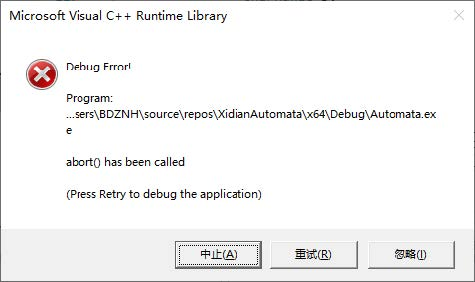
\includegraphics[width=0.60\textwidth]{DFA_usefulf_error}
    \caption{函数 DFA::usefulf() 错误提示}
    \label{fig::usefulf_error}
\end{figure}
控制台提示如图 \ref{fig::usefulf_console_log}
\begin{figure}[!htbp]
    \centering
    %trim option's parameter order: left bottom right top
    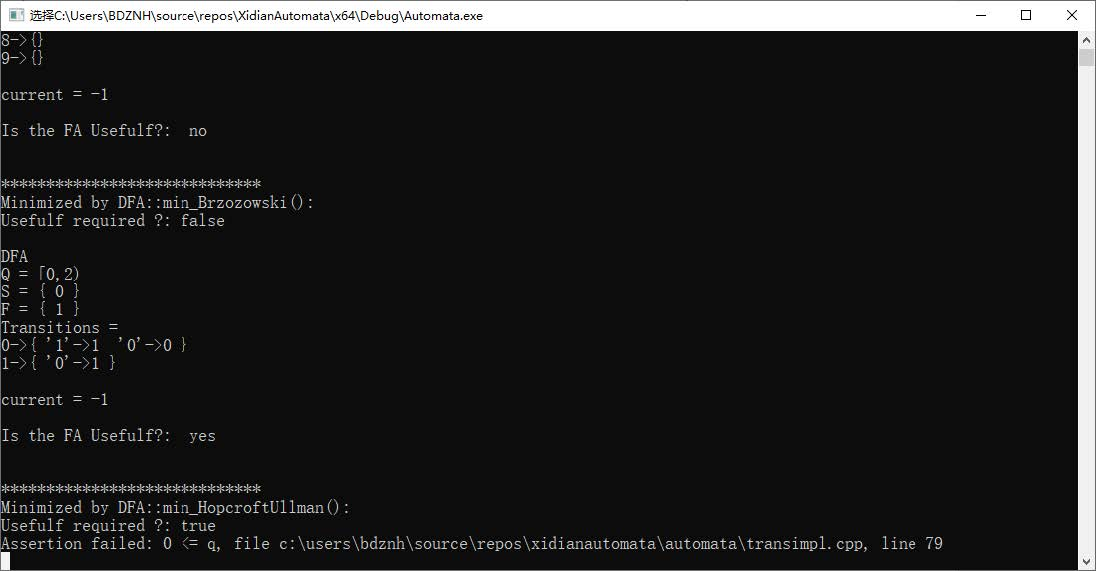
\includegraphics[trim = 0mm 0mm 0mm 63mm, clip,width=0.95\textwidth]{DFA_usefulf_console_log}
    \caption{函数 DFA::usefulf() 错误提示}
    \label{fig::usefulf_console_log}
\end{figure}

可以确定函数为完成其定义功能。

%%%%%%%%%%%%%%%%%%%%%%%%%%%%%%%%%%%%%%%%%%%%%%%%%%%%%%%%%%%%%%%%%%%%%%%%%%%%%%%%%%%%%%%%%%%%%%%%%%%%%%%%%%%%%%%%%%%%%%%%%%%%%%%%%%%%%%%%%%%%%%%%%%%%%%%%%%%%%%%%%%%%%%%%%%%%%
% {\bfseries 错误原因}
\subsection{错误原因}

查看 TransImple.cpp,79行,代码如下
\lstset{style=mystyle}
\begin{lstlisting}[language=C++,label={lst:TransImple},caption={ TransImple.cpp },firstnumber=75]
// Add a transition to the set.
TransImpl& TransImpl::add_transition(const CharRange a, const State q)
{
    assert(a.class_invariant());
    assert(0 <= q);
    ………
}
\end{lstlisting}

在 79 行处打断点,单步调试至此处,可以看到 State 变量 q 的值为“-842150451”,对应的十六进制值为“0xFFFFFFFF”\footnote{调试时使用 64 位编译器产生的二进制文件,在 64 位系统下运行。},为常见的未初始化错误。此时表达式 “0 <= q” 不成立,返回值为 “false” , 程序在此处中止。

查看函数 DFA::usefulf() 的实现,如代码 \ref{lst:DFA_usefulf_1} 。
\lstset{style=mystyle}
\begin{lstlisting}[language=C++,label={lst:DFA_usefulf_1},caption={ DFA.cpp },firstnumber=84]
StateTo<State> newnames;
newnames.set_domain(Q.size());

// All components will be constructed into a special structure :
DFA_components ret;
State st;
for (st = 0; st < Q.size(); st++)
{
    // If this is a Usefulf State, carry it over by giving it a name
    // in the new DFA.
    if (freachable.contains(st))
    {
        newnames.map(st) = ret.Q.allocate();
    }
}
\end{lstlisting}
在代码 \ref{lst:DFA_usefulf_1} 中将 “ final-reachable ” 状态保存到 StateTo<State> 变量 newnames 中,通过 “ ret.Q.allocate()” 为状态命名新的状态名,作为新的自动机的状态名。DFA\_components 变量 ret 用于构建新的自动机,再看函数内构造新的自动机的主要实现部分,如代码 \ref{lst:DFA_usefulf_2}
\lstset{style=mystyle}
\begin{lstlisting}[language=C++,label={lst:DFA_usefulf_2},caption={ DFA.cpp },firstnumber=115]
CRSet a;
for (State st = 0; st < Q.size(); st++)
{
    // If st is the representative, construct the transition.
    if (st == r.eq_class_representative(st))
    {
        State stprime(newnames.lookup(st));
        // What are st's out-transitions?
        CharRange b;
        a = T.out_labels(st);
        // The out-labels of any other element of [st]_r could have
        // been used instead. Some other choice may, indeed, lead
        // to a smaller DFA.This approach is used for simplicity.
        int it;
        // Iterate over the labels, constructing the transitions.
        for (it = 0; !a.iter_end(it); it++)
        {
            b = a.iterator(it);
            ret.T.add_transition(stprime, b, newnames.lookup(T.transition_on_range(st, b)));
        }
    // st's eq. class may be final.
    if (F.contains(st)) ret.F.add(stprime);
    }
}
\end{lstlisting}

根据代码 \ref{lst:TransImple} ,可以知道程序中止的地方为代码 \ref{lst:DFA_usefulf_2},134 行。其中 State 变量为当前需要进行操作的状态,CharRange 变量 b 为当前状态转移输入字符。查看 T.
transition\_on\_range(st, b)) 的实现,如代码 \ref{lst:transition_on_range}
\lstset{style=mystyle}
\begin{lstlisting}[language=C++,label={lst:transition_on_range},caption={ DTransRel.cpp },firstnumber=108]
// Compute the image of r, and CharRange it under *this.
inline State DTransRel::transition_on_range(const State r, const CharRange a) const
{
    assert(class_invariant());
    assert(0 <= r && r < domain());
    return(lookup(r).range_transition(a));
}
\end{lstlisting}
由代码 \ref{lst:transition_on_range} 可知,T.transition\_on\_range(st, b)) 将返回原自动机中,状态 st 经过输入字符 b 转移之后的目标状态。

查看 newnames.lookup() 的实现,如代码 \ref{lst:newnames-lookup}
\lstset{style=mystyle}
\begin{lstlisting}[language=C++,label={lst:newnames-lookup},caption={ StateTo.h },firstnumber=177]
// The actual mapping function
// First, a const lookup operator.
template<class T>
inline const T& StateTo<T>::lookup(const State r) const
{
    assert(class_invariant());
    // First check that it's in bounds
    assert(0 <= r && r < domain());
    return(data[r]);
}
\end{lstlisting}
在本例中,模板类 StateTo<T> 的模板参数 “T” 为 State。则 newnames.lookup(T.transition\_on\_range(st, b)) 为原自动机中 状态 st 经过字符 b 转移后的目标状态在新自动机中的状态。然后通过 ret.T.add\_transition() 保存新的转移关系。对所有的状态进行以上操作之后,通过变量 ret 构造新的自动机。 

经过单步调试发现,表\ref{tab:DFA4} 中,状态 $q_2$ 经过字符 “1” 将转移到状态 $q_5$,而在代码 \ref{lst:DFA_usefulf_1} 中,状态 $q_5$ 不满足 “if (freachable.contains(st))”,所以状态 $q_5$ 未被新的自动机保存,进而在代码 \ref{lst:DFA_usefulf_2} 中,当 st 为状态 $q_2$ 且 b 为字符 “1” 时,“newnames.lookup(T.transition\_on\_range(st, b))” 将返回未经初始化的值“-842150451”,于是在代码 \ref{lst:TransImple} 中,State 变量 q 的值为“-842150451”,导致程序在此处中止。

%%%%%%%%%%%%%%%%%%%%%%%%%%%%%%%%%%%%%%%%%%%%%%%%%%%%%%%%%%%%%%%%%%%%%%%%%%%%%%%%%%%%%%%%%%%%%%%%%%%%%%%%%%%%%%%%%%%%%%%%
\subsection{解决方法}

如代码 \ref{lst:State_H} 所示,文件 State.h 中将无效状态设置为 “Invalid”。在代码 \ref{lst:DFA_usefulf_1}增加处理不满足条件 “freachable.contains(st)” 的状态的内容,将原自动机中的非“final-reachable”状态标记为 “Invalid”,更改后为代码 \ref{lst:DFA_usefulf_1_edit}
\lstset{style=mystyle}
\begin{lstlisting}[language=C++,label={lst:DFA_usefulf_1_edit},caption={ 更改后的 DFA.cpp },firstnumber=91]
for (st = 0; st < Q.size(); st++)
{
    // If this is a Usefulf State, carry it over by giving it a name
    // in the new DFA.
    if (freachable.contains(st))
    {
        newnames.map(st) = ret.Q.allocate();
    }
    else                            // 新增
    {                               // 新增
        newnames.map(st) = Invalid; // 新增
    }                               // 新增
}
\end{lstlisting}

在代码 \ref{lst:DFA_usefulf_2} 中,在添加新的转移关系之前判断状态是否都是有效状态,更改后为代码 \ref{lst:DFA_usefulf_2_edit}
\lstset{style=mystyle}
\begin{lstlisting}[language=C++,label={lst:DFA_usefulf_2_edit},caption={ 更改后的 DFA.cpp },firstnumber=133]
    State stdest;                                           // 新增
    stdest = newnames.lookup(T.transition_on_range(st, b)); // 新增

    if (stprime != Invalid &&  stdest != Invalid)           // 新增
    {                                                       // 新增
        ret.T.add_transition(stprime, b, stdest));          // 更改
    }                                                       // 新增
\end{lstlisting}

更改后函数 DFA::usefulf() 成功将图 \ref{fig:DFA4_0} 转换成图 \ref{fig:DFA4_1} 。

\section{函数 DFA::min\_opcroft() 运行结果错误}